
\section{Introduction/Motivation}

\quad Yelp is a website which allows users to create an account and review businesses. Our goal is to analyze data from Yelp to gain further insight for business owners to develop a more satisfactory experience for their customers. Yelp has a large public dataset available on their website with information about users, businesses, and reviews.

\quad Our first objective is to determine if certain attributes are indicative of business success with respect to their average review rating (see sec. 2.3 for revenue relation). For the businesses with many reviews, time-series data of the average star rating of the business mined from user reviews can be analyzed with ML models like Hidden Markov Models or recurrent neural networks in order to learn the likelihood of a business failing or succeeding in the future based on its current ratings. Furthermore, sentiment analysis can be used on language of reviews and matched with the star reviews to provide more information on a business?s chances of success. Additionally, information about the current state of a business and likely future states could be provided to businesses to permit them to change their current practices and focus to increase their chances of success.

\quad Another way sentiment analysis will prove helpful in this project is to analyze the emotions conveyed by the reviewer as being pleased or angry at their experience with the business. Using the results of this analysis we hope to be able to determine if certain times of day, city locations, or other factors contribute to the experience of a customer. This information could also contribute to a business model. As an example, if certain locations are more prone to angry customers it could indicate that the people in that area have high standards, the businesses are poorly run, or just that those customers tend to leave angry reviews. This type of information will be less useful to businesses, but it could prove very helpful for customers or advertisers to know that businesses in a certain area tend to be reviewed much higher or lower than the average business in cities of a comparable size.

\quad Our last objective is to find recurring problems in businesses. With natural language processing tools, we can analyze review text to find the specific issues that people are having with businesses via keywords or repeated references to specific aspects of the business. Again, this will be most helpful in analyzing reviews for businesses with many reviews. If one of these businesses has many reviews which all indicate a similar issue, then that is useful information that a business owner would want to be aware of so that they can eliminate the problem, if possible.

% Head 1
\section{Prior Work}

Since our problem involves predictions surrounding businesses, we sought out similar research to guide our investigation. Thus, we focus our literature review on studies that utilized some form of sentiment analysis, constructed predictive models, and/or conducted meta-analysis of trends in the aforementioned sentiment, rating, or business interest.

% Head 2
\subsection{Predicting Business Attention}

A previous winner, Hood et al., published a paper on assessing a business?s current rating/review state and future expectations with respect to review numbers on Yelp. The bulk of their work centered around the creation of additional features for the data (e.g. number of similar businesses within 1km, features of subsets of reviews such as average rating and number of unique users). From there they utilized various feature reduction and clustering techniques to build a prediction model. They were able to identify features that offered greater accuracy in prediction of interest in the business (calculated as the predicted number of reviews within 6 months after a target date) as well as a create model for prediction that outperformed a basic linear regression. Our approach will be similar in the application of feature reduction to reduce the dimensions of that data and clustering to find cities with many businesses, as well as to group similar businesses together. However, we do not plan to create additional features like the number of nearby similar businesses.

% Head 3
\subsection{Latent Subtopics}

Huang et al. (2013) utilized probabilistic models to discover underlying subtopics within Yelp reviews. This offered a framework to categorize the reviews based on review text. From here, they were able to analyze the prevalence of various star ratings within each category. In this way, they could advise business owners as to the common trends among good and bad reviews that may not be apparent without considering the review text. McAuley and Leskovec built on this idea by combining such latent review topics with hidden rating driving factors, allowing them construct a rating prediction model.

\subsection{Reviews and Revenue}

In one of the more influential papers on the subject, Michael Luca showed a correlation between Yelp rating and revenue, highlighting the fact that rounding to half stars could significantly impact two similarly-rated restaurants if their averages fell on either side of the divide (e.g. 3.24 and 3.26). He goes on to build a model of market response based on review volume as well as the impact of user expertise. He concluded that such responses are consistent with a Bayesian learning model.

\section{Proposed Work and Dataset Information}

\subsection{Proposed Work}

The dataset has many optional attributes. There is an attribute simply called 'attributes' that is a shopping list of optional fields for each business. This part of the dataset is inconsistent and the same fields cannot be relied upon to be present for each business. For instance, one of these attributes is 'Bike Parking.' This attribute is either true, false, or nonexistent. In the cases when it is nonexistent, analysis based upon this attribute is obviously unreliable. Most of these miscellaneous attributes are present for much less than a majority of the data, so any mining based upon them would have to first drastically trim the data available for analysis by eliminating more than half the data. For this reason, we have chosen to eliminate the miscellaneous category rather than most of our data.

\quad In addition, the data is not only restaurants but many kinds of businesses. A datum associated with each business attempts to classify the business as a member of a category, such as ?restaurants,? ?beaches,? or ?shopping.? However some categories are extremely broad and the same type of business can be described in different ways. One example is that a bakery may be classified as belonging to ?bakeries,? but also generically as ?food.? Conversely, many businesses sell food, but the generic category ?food? will not be in their list of categories and instead the business will be labelled with more specific categories like ?Italian food,? diminishing the usefulness of these categories.

\quad The dataset provided by the Yelp organizers is fairly clean already, and the majority of the data cleaning process will be involved in handling missing data. It is possible to fill in these missing values with default values like ?false?, or ?none? but it can be dangerous to make assumptions about what businesses have and don?t have - for example, filling in a ?gluten-free? attribute of a business may influence our analysis of its reviews and, depending on exposure, maybe even mislead Yelp users as to what the business provides.

\quad The Yelp dataset contains up to a million different attributes about businesses from 11 different cities in 4 countries. The majority of these attributes will be unnecessary so there will be a large effort in data reduction. For instance, the dataset includes photographs of the exterior and interior of some businesses (also many images of various kinds of food served by the businesses), but our questions does not require image analysis. There also redundant attributes such as postal codes that are unnecessary because latitude and longitude is more accurate.

\subsection{Dataset}

The Yelp dataset comes from the Yelp Dataset Challenge. This is an ongoing challenge and this is the ninth round, so the challenge is very well-established by this point. The challenge offers \$5,000 to the winner and the final submission takes the form of an academic paper.

\quad We will be considering the following from the Yelp dataset:

\begin{itemize}
	\item{4.1 million reviews}
	\begin{verbatim}
	"review_id":(encrypted review id),
	"user_id":(encrypted user id),
	"business_id":(encrypted business id)"
	"stars":(star rating, rounded to half-stars),
	"date":(date, formatted: YYYY-MM-DD),
	"text":"review text",
	"useful":('useful' vote count),
	"funny":('funny' vote count),
	"cool": ('cool' vote count),
	"type": "review"
	\end{verbatim}
	\item{Information on 144,000 businesses in 11 cities from 4 countries (incl. the US, Germany, Canada, and the U.K. (with 1.1 million business attributes)}
	\begin{verbatim}
	"business_id":(encrypted business id),
	"name":"business name",
	"neighborhood": "hood name",
	"address":"full address",
	"city":"city",
	"state":"state"(if applicable),
	"postal code":"postal code",
	"latitude":latitude,
	"longitude":longitude,
	"stars":(star rating, rounded to half-stars),
	"review_count":(number of reviews),
	"is_open":0/1 (closed/open),
	"attributes":[(localized attribute tags)],
	"categories":[(localized category names)],
	"hours":[(hours strings)],
	"type": "business"
	\end{verbatim}
	\item{Over 1M users}
	\begin{verbatim}
	"user_id":(encrypted user id),
	"name":"first name",
	"review_count":(number of reviews),
	"yelping_since": (date, formatted: YYYY-MM-DD),
	"friends":[(encrypted user ids)],
	"useful":('useful' vote count sent by user),
	"funny":('funny' vote count sent by user),
	"cool": ('cool' vote count sent by user),
	"fans":"number of fans the user has",
	"elite":["an array of years the user was elite"],
	"average_stars":floating point average like 4.31,
	"compliment_type": (compliment count),
		...(same for each complement type)...
	"type":"user"
	\end{verbatim}
	\item{Over 200,000 user-submitted photographs, 947,000 tips, and aggregated check-in data for most businesses}
\end{itemize}

\section{Methods and Tools}

\quad The tools and methods used for this project will no longer include a database for storing or integrating the data. Due to difficulties described in section 6 and relating to the unknown JSON variant used by the preparers of the Yelp dataset, storing the data in a database is not feasible at this time. Given that the data is already quite clean save for the format, with minimal replacement of missing values and some other changes necessary, it is possible for each group member to have a copy of the data stored locally that may be processed with our tools, with smaller subsets of data, results, and scripts shared via GitHub. The datasets will be merged locally, and while this does increase the amount of computational work necessary for each member?s machine, the dataset is still of a small enough size (less than 10 GB, excluding the photos) that this is practical. We will still use various Python libraries and modules for cleaning and preprocessing, and various other tools for transformation, mining, pattern evaluation, and knowledge presentation. The lack of a centralized database in removes the need for a number of Python libraries like Dora and FTFY ('fixes text for you') intended for data cleaning and preprocessing, but increases the necessity of group communication to reduce duplication of work and miscommunications. We currently use and will continue to use Slack, email, and in-person meetings to communicate and synchronize our efforts. 

\quad Numpy, Scipy, and Pandas will be used to transform and mine the data, and other Python modules like Seaborn and Plotly (a Python API for D3) will be used for knowledge visualization and presentation. Rather than relying on tools like Weka, the Text Analytics API from Microsoft Cognitive Services, or the Facebook fastText pre-trained word vectors, we will instead use Python?s Natural Language Toolkit for sentiment analysis and other language processing.


\section{Evaluation}

\subsection{Methodology}

\quad Evaluating our predictions as to whether a business success will hinge on comparing the star rating (from one to five stars) and our predicted star rating based on the other attributes in the review, such as day of the week and month, season, or location. This could be done by training an ML algorithm like Kernel Ridge regression on 80\% of the data and testing it on the remaining 20\%, and then adjusting parameters to minimize the error between the actual star ratings and our predicted star ratings for the testing data.

\quad Also, evaluating the sentiment analysis of the review text will likely be simple given that we will be using tools like NLTK (see following section) to perform sentiment analysis rather than creating entirely custom algorithms. These tools incorporate helpful metrics to analyze the error of a particular output. Alternatively, we can manually verify the sentiment of a (relatively small) number of reviews by reading them and comparing our human judgements of the sentiment to the output of the tools. For evaluating recurring problems, we will employ a similar approach, except we will group reviews by business and analyze them as a time series to and recurring issues. For recurring problems specifically, the most expedient method of evaluation may well be to read a small number of reviews and manually determine evaluate the performance of our tools in detecting recurrent issues.

\quad For all three of the objective questions, employing association rule frameworks that use support-confidence frameworks will be helpful to find and measure strong associations, while null-invariant measures like the Kulczynski measure or the cosine measure will be helpful to determine how interesting these associations are.

\section{Progress}

There have been several major changes to the project tools and methods since the project proposal. Initially we planned on using a relational database to store, integrate, and access the data, but but we encountered many difficulties in just uploading the data. The inconsistencies between the user and business data made it exceedingly difficult to successfully import the data en masse into the database, so instead we decided to import the data straight into Weka. However, the format of the JSON file also did not allow a successful import into Weka. 

\quad Next we converted the JSON file into CSV format using a Python script and tried to upload it to Weka again. Once again Weka had issues due to the mismatch in attributes for each business (some had more attributes while others had less, likely due to the ?miscellaneous? category mentioned in section 3.1).

\quad Instead we opted to use a different tool, RapidMiner. Like Weka, RapidMiner incorporates extensive machine learning functionality like classification, regression, clustering, and association and frequent itemset mining. RapidMiner is commercial software, but an educational version is available that removes certain limitations on the free version like only being able to process 10,000 rows at a time. Additionally, RapidMiner is much more compatible with the missing data in our dataset and automatically corrects the formatting issues we had when attempting to use Weka. It does not support JSON so we reused the conversion code (found on the team GitHub as convert.py) to convert the data files to CSV. 

\section{Results}

\subsection{Businesses}

After importing the CSV version of the data, we tested some basic visualization tools from RapidMiner. For instance, in Figure 1 we created a histogram of the average star for a business versus the state in which it is located. Basic graphs like these can help refine our questions. For example, why does Illinois have significantly lower average stars than other states or provinces, even those that border it? 

\quad The most pervasive issue with our business data is that many entries are missing data, most notably the miscellaneous 'attributes' and address information. Since these values are managed by the account owner, they vary widely across the businesses. However, some of these data are redundant given the other fields, such as detailed latitude-longitude data for each business.

\begin{figure}[h]
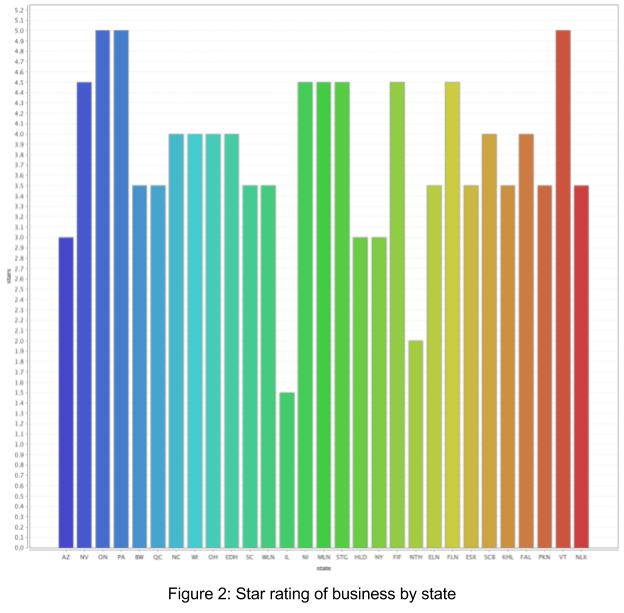
\includegraphics[width=0.75\textwidth, center]{b_rating_by_state}
\end{figure}

RapidMiner can also produce 3D scatterplots which is useful because we plan to use latitude and longitude to locate businesses, since some of the business address data is missing and cannot (and should not) be replaced with default values or other common values used to replace missing data. Figure 2 depicts a graph of longitude vs. latitude vs. review count for businesses. 

\begin{figure}[!h]
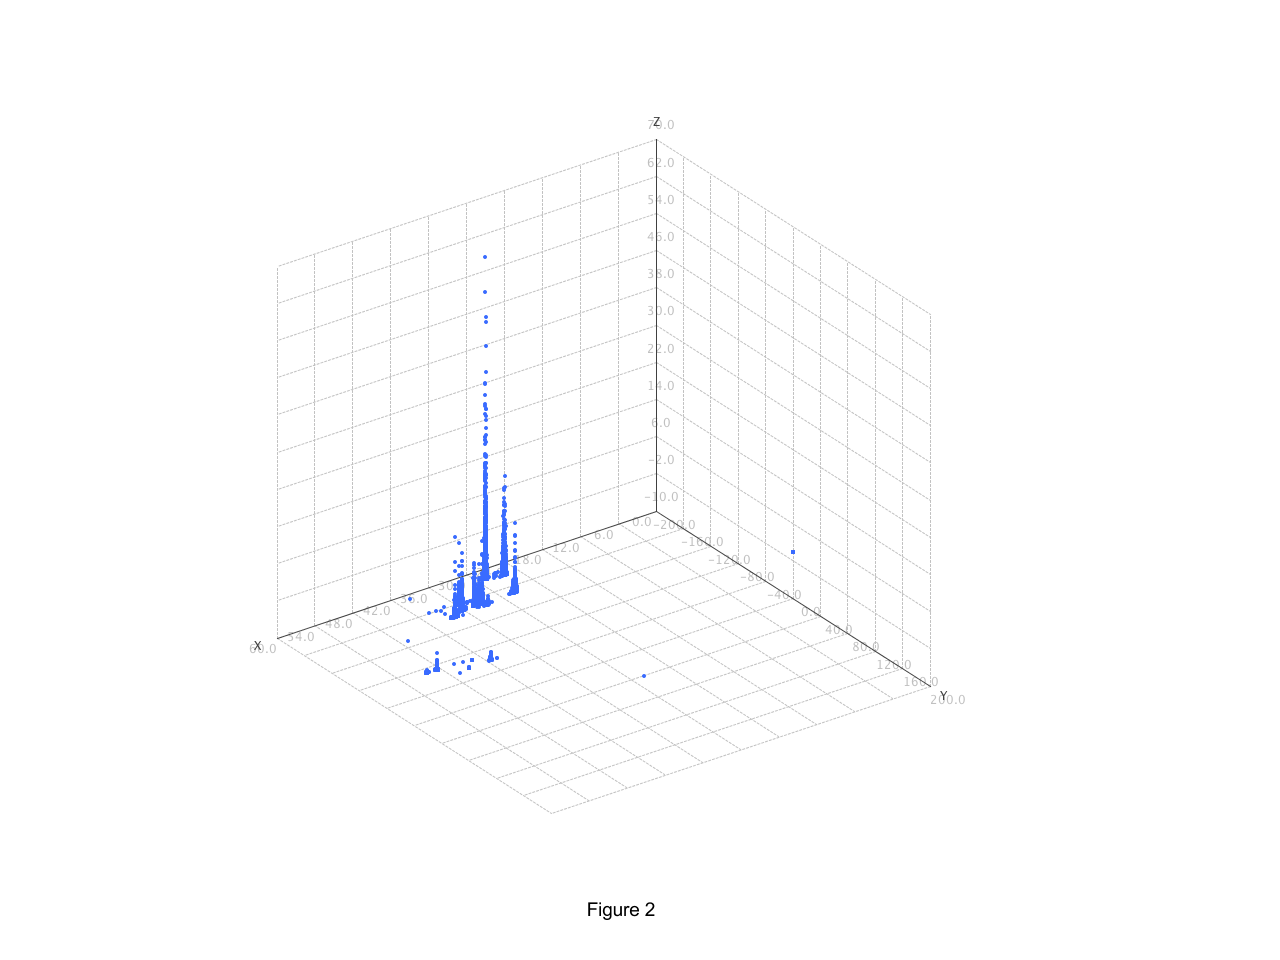
\includegraphics[width=0.75\textwidth, center]{3d_businesses_lat_long}
\end{figure}

In this instance the visualization makes it clear that reviews are more frequent in populated cities as we expect. However, it also shows visually the outliers. There are various businesses that have only a few reviews. In this context it is easier to identify outliers and also see that businesses concentrate in certain locations, as is expected given Yelp?s declaration that the dataset focuses on businesses in 11 cities. Therefore we can reduce the dataset to only the cities that meet the threshold of businesses or total review counts. 

\subsection{Business Categories}
    \quad In an effort to garner more information about user behavior, we needed to augment the initial data with that from the businesses and reviews, the latter of which serves as the link between the former two. In doing so, we attempted to profile the most frequent business reviewed by each user. The two troublesome business features were the user-defined ?tags? and ?categories?. The categories proved to be a more manageable problem as they are selected from a finite set of options. With numbers of selected categories ranging from two to twenty-eight out of over 1000 possible choices, we sought to reduce this high degree of dimensionality.
    \quad Sparse binary data of this kind quickly becomes unwieldy as traditional distance measures are highly prone to error. Such measures include K-Means, PCA analysis (for dimensionality reduction), DBSCAN, and Agglomerative Clustering. Typically, the computational cost is prohibitive (Plumpley, et. al., 2002) or the numerical values are highly unstable during computation. The goal in our application is to reduce the effective categorical space and classify the businesses into a narrower subset?on the order of ~50. Not surprisingly, this scenario is almost identical to that encountered when processing and analyzing large corpuses of text. Almost every form of textual representation falls into the ?bag-of-words? paradigm where vectors are used to represent each document, and each element corresponds to either the frequency of a given term in the dictionary (i.e. all words from all documents) or the binary existence of the word in the document. Since each document is highly unlikely to have an instance of all terms, the combination of these vectors results in a very large, very sparse matrix of n documents by p terms.
    \quad Much research has been done in recent years on Latent Semantic Analysis (or Indexing). This utilizes the fact that a given matrix?s Singular Value Decomposition provides us with a large degree of useful data concerning the nature of the matrix, namely which vectors and rows carry more weight as well as those with less impact. Furthermore, it provides a model through which new data can be projected onto the reduced subspace. The table below shows a sample of the reduced vector space and the first ten terms in each of the new topics.

\subsection{Reviews}

One of the major goals of the project is to find recurrent problems and other issues with the businesses, and this was to be done by grouping reviews by business and then analyzing trends in the language used in the reviews over time. However, given that we were unable to find a suitable workaround for our difficulties with Weka, we used sentiment analysis tools from the Natural Language Toolkit (NLTK) to analyze the review language instead. NLTK is a language-processing and analysis platform that uses Python, and a good replacement for the language processing capabilities of Weka. 

\quad Using a custom script (see GitHub\; nltk\_review\_subset\_process.py) to analyze the sentiment of the first 100,000 reviews (about 2.5\% of the available data), we discovered that the average sentiment score among all analyzed reviews was around 0.113, and there were 17295 negative reviews compared to 76968 positive reviews. The remaining 5737 reviews had composite sentiment scores within -0.2 < score < 0.2, so they were excluded from further analysis since they were neutral. This means that the average Yelp review (at least within the analyzed subset) is positive rather than negative or neutral in sentiment, perhaps indicating that Yelp users are more inclined to write reviews of businesses with which they had a good experience. Only around 2.5\% of the data is currently processed by the file, because processing the entire file is prohibitively expensive.

\subsection{Users}

The users dataset essentially provides a window into users' status, connections, and interaction within the Yelp ecosystem. The figure below shows a plot of the user data. We see that the user density grows around 3.25-4.25 average rating with some traces of a bell curve regarding the number of reviews.

\begin{figure}[!h]
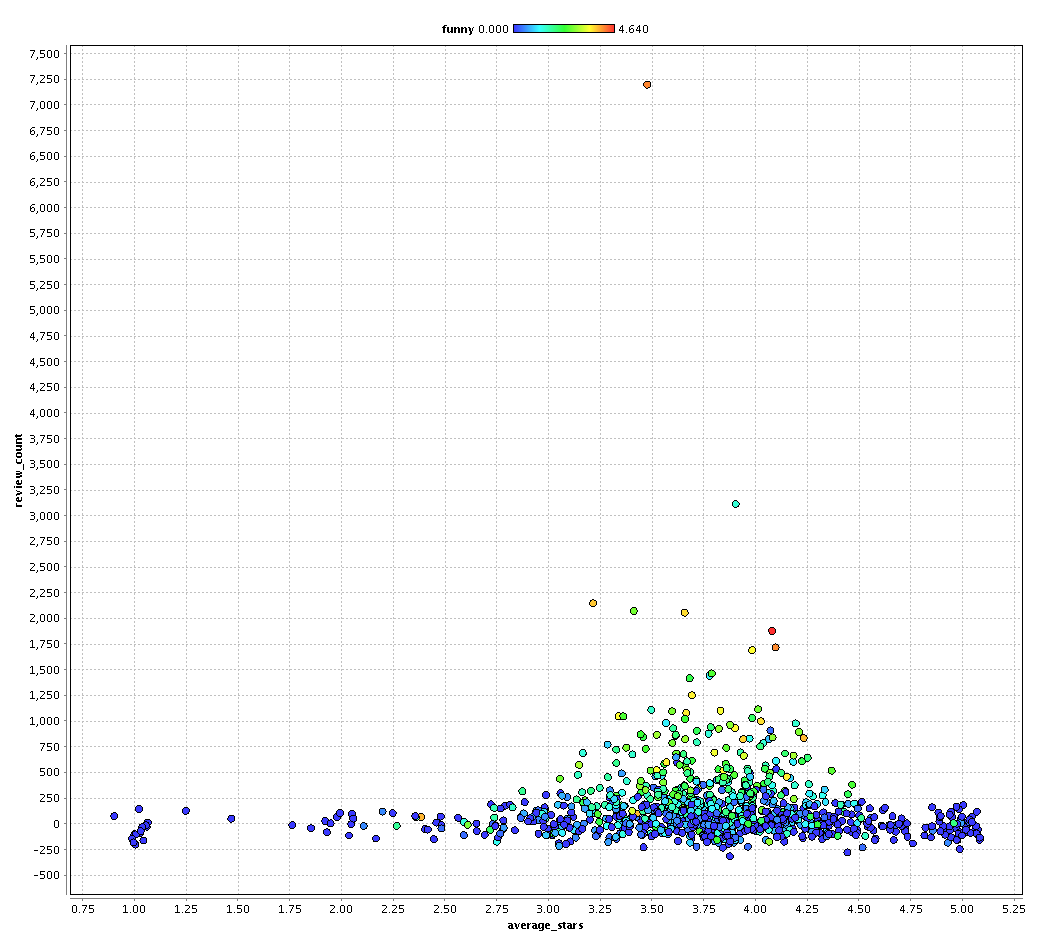
\includegraphics[width=0.45\textwidth, center]{u_reviews_vs_stars}
\end{figure}

\quad One of the most significant yet hardest to process attributes is the 'friends' list. This attribute provides an opportunity to model our data as a graph. Such a network could provide very relevant clustering through sparseness measures and cutting in addition to accounting for user/business influence or finding deeper trends according to network connectivity. However, given the magnitude of the dataset, modeling the ?friends? of each user as a complete graph will be computationally difficult. To combat this, we could limit our model to the first n people the graph builder encounters only, since connections between groups of people are unpredictable.

\quad
\section{Next Steps}

\quad It is still necessary to reduce dimensionality. We've currently been working on the whole dataset and simply ignoring all attributes that fall in the category 'other.' This is cumbersome and it will become increasingly detrimental as we use more advanced techniques like clustering. The most prioritized attribute is the attributes portion. This attribute has the most issues because it is a miscellaneous catch-all where any attribute that didn?t fit with the others is thrown in. The issue is that it totally lacks consistency in the number and types of miscellaneous attributes included for each business. One business may have a Free Wifi attribute while others may not. After looking through the data it was clear that there wasn?t one attribute in this misc. category that was reliably present for all businesses. Although we have moved on to work with the other attributes, this one still needs work to decide if it should be omitted completely or if default values should be set instead.

\quad In addition, we need to combine the businesses and reviews dataset. This becomes extremely useful when examining the sentiment of a review and finding a correlation with the attributes of a business. This helps us build a model to potentially predict if a business receives negative or positive reviews based on its attributes. 

\quad As mentioned before, we will be interested in clustering businesses together as to whether they receive positive or negative reviews based on their attributes. This can be difficult with the high number of dimensions of these datasets. We will try CLIQUE and PROCLUS for subspace clustering. PROCLUS will be particularly useful because the subspace for one business to qualify as ?positively reviewed? could be different than the subspace for another business. This allows us to process this data faster, but also consider the complexities of various subspaces. 

\quad The user and review datasets are the largest we have. We would like to use these to find useful information about the people and the reviews they give. Because Yelp is a platform on which anybody can create an account and write a review, it is possible that not everybody is honest and fair in their reviews. Furthermore, different people may assign scores for different reasons. 

\quad Some useful attributes in the user data alone are the number of reviews that an individual has made, the length of time a user has been active on Yelp, and whether their reviews tend to be tagged as useful by other users. 

\quad One additional consideration is processing power. Our chosen tool seems to be very computationally intensive, so we will very likely need to use sampled data to test hypotheses then turn to python scripts to actually run over the entirety of our training, testing, and validations sets. Furthermore, our data is currently only linked through review, user, and business id pointers. While there?s a great deal to be learned from each collection individually, we will need to connect our disparate sets by these terms. 

\quad Currently, the review dataset is too large to process in detail. In the future, we will continue taking subset samples of a more reasonable size and processing those instead, as well as increasing the complexity of our analysis. Combining the review dataset with the business dataset (using the 'business\_id' field as a key) will enable us to produce maps of where the largest number of reviews with negative and positive sentiment are, as well as seeing where users leave the most strongly-worded reviews. We hope that additional advanced sentiment analysis will be useful in determining underlying factors that influence a business's success, as well as in identifying recurrent problems.

\quad Once we have our sentiment analysis we can combine this data with our user data and business data to find patterns in the sentiment of reviews. We would like to compare the sentiment of reviews to the area they are coming from, the businesses they apply to, and whether reviews of a given sentiment are considered beneficial by other users. Using this information we can then narrow down the factors that are most influential to the score of a business in order to draw our final conclusions.


% Start of "Sample References" section

%\section{Typical references in new ACM Reference Format}
%A paginated journal article \cite{Abril07}, an enumerated
%journal article \cite{Cohen07}, a reference to an entire issue \cite{JCohen96},
%a monograph (whole book) \cite{Kosiur01}, a monograph/whole book in a series (see 2a in spec. document)
%\cite{Harel79}, a divisible-book such as an anthology or compilation \cite{Editor00}
%followed by the same example, however we only output the series if the volume number is given
%\cite{Editor00a} (so Editor00a's series should NOT be present since it has no vol. no.),
%a chapter in a divisible book \cite{Spector90}, a chapter in a divisible book
%in a series \cite{Douglass98}, a multi-volume work as book \cite{Knuth97},
%an article in a proceedings (of a conference, symposium, workshop for example)
%(paginated proceedings article) \cite{Andler79}, a proceedings article
%with all possible elements \cite{Smith10}, an example of an enumerated
%proceedings article \cite{VanGundy07},
%an informally published work \cite{Harel78}, a doctoral dissertation \cite{Clarkson85},
%a master's thesis: \cite{anisi03}, an online document / world wide web
%resource \cite{Thornburg01, Ablamowicz07, Poker06}, a video game (Case 1) \cite{Obama08} and (Case 2) \cite{Novak03}
%and \cite{Lee05} and (Case 3) a patent \cite{JoeScientist001},
%work accepted for publication \cite{rous08}, 'YYYYb'-test for prolific author
%\cite{SaeediMEJ10} and \cite{SaeediJETC10}. Other cites might contain
%'duplicate' DOI and URLs (some SIAM articles) \cite{Kirschmer:2010:AEI:1958016.1958018}.
%Boris / Barbara Beeton: multi-volume works as books
%\cite{MR781536} and \cite{MR781537}.
%
%A couple of citations with DOIs: \cite{2004:ITE:1009386.1010128,
%  Kirschmer:2010:AEI:1958016.1958018}. 

% Bibliography
\bibliographystyle{ACM-Reference-Format}
\bibliography{sample-bibliography}
